\section{IO Board}
\index{IO Board}
The V6 webbrick comes with an IO board that provides screw terminal access to all connections other than the 
network cable. It also provides 4 switched mains outputs and 2 double pole changeover relay outputs.

Layout diagram In here.

\subsection{Mains Switching}
\index{Mains Switching}
The mains outputs are digital channels 1 to 4 and can each switch up to 500W, with a maximum of 1500W for the four channels.
There is a 6.3 Amp fuse in the unit that will blow if you excede this loading. These are zero voltage switched and intended 
for simple on off actions. To handle dimming use the analogue outputs connected to external dimmers.

\subsection{Relays}
\index{Relays}
Digital channels 4 and 5 are connected to relays that provide a double pole changeover capability and are rated for 4A at 230V. 

\em{6 Series} Due to internal spacing these should not be used for low voltage applications if the mains switching capability is 
used on the Triacs.

\em{7 Series} The relays are now organised so that relay 5 is a double pole changeover and relay 4 is presented as single pole changeover.  
Internally the connections for relay 4 are paralleled.  This gives a current rating of 4A at 230V for relay 5 and 8A at 230V for relay 4.

The arrangement of the live side protective ground has been changed so that low voltages can be used on the relays whilst mains is present on the triacs. 



\subsection{Connections}
\index{Connections}

The IO board has a total of 6 connectors on it, 2 are 9 way and 4 are 12 way. The 9 way connectors are used for the 
mains outputs and the 12 way for inputs and low voltage outputs.

\begin{figure}[H]
\centering
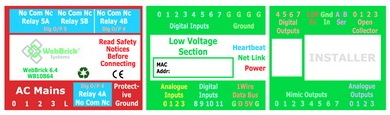
\includegraphics[width=0.6\textwidth]{Images/TopCover.jpg}
\caption{WebBrick IO connectors}
\end{figure}

\begin{tabular}{l|p{5cm}}
Connector X1&Relay connections\\
\hline
Pin 1&Mains Triac 0\\
Pin 2&Mains Triac 1\\
Pin 3&Mains Triac 2\\
Pin 4&Mains Triac 3\\
Pin 5&Mains In\\
Pin 6&Relay1 NO1\\
Pin 7&Relay1 C1\\
Pin 8&Relay1 NC1\\
Pin 9&Mains Earth\\
\end{tabular}

\begin{tabular}{l|p{5cm}}
Connector X2&Triac/Mains and more Relay connections\\
\hline
Pin 1&Relay1 NO2\\
Pin 2&Relay1 C2\\
Pin 3&Relay1 NC2\\
Pin 4&Relay2 NO1\\
Pin 5&Relay2 C1\\
Pin 6&Relay2 NC1\\
Pin 7&Relay2 NO2\\
Pin 8&Relay2 C2\\
Pin 9&Relay2 NC2\\
\end{tabular}

\begin{tabular}{l|p{5cm}}
Connector U1&\\
\hline
Pin 1&0V-Digital Ground\\
Pin 2&0V-Digital Ground\\
Pin 3&0V-Digital Ground\\
Pin 4&0V-Digital Ground\\
Pin 5&Digital In 7\\
Pin 6&Digital In 6\\
Pin 7&Digital In 5\\
Pin 8&Digital In 4\\
Pin 9&Digital In 3\\
Pin 10&Digital In 2\\
Pin 11&Digital In 1\\
Pin 12&Digital In 0\\
\end{tabular}

\begin{tabular}{l|p{5cm}}
Connector U2&\\
\hline
Pin 1&Analogue In 0\\
Pin 2&Analogue In 1\\
Pin 3&Analogue In 2\\
Pin 4&Analogue In 3\\
Pin 5&Digital Input 8 - may be labelled Digital Monitor 1\\
Pin 6&Digital Input 9 - may be labelled Digital Monitor 2\\
Pin 7&Digital Input 10 - may be labelled Digital Monitor 3\\
Pin 8&Digital Input 11 - may be labelled Digital Monitor 4\& IR In\\
Pin 9&0V-Digital Ground\\
Pin 10&1 Wire data bus\\
Pin 11&1 Wire 5V Supply\\
Pin 12&0V-Digital Ground\\
\end{tabular}

\begin{tabular}{l|p{5cm}}
Connector U3&\\
\hline
Pin 1&Open Collector Digital 0\\
Pin 2&Open Collector Digital 1\\
Pin 3&Open Collector Digital 2\\
Pin 4&Open Collector Digital 3\\
Pin 5&Special Connection A\\
Pin 6&Special Connection B\\
Pin 7&0V-Digital Ground\\
Pin 8&12V Supply In\\
Pin 9&Digital 4\\
Pin 10&Digital 5\\
Pin 11&Digital 6\\
Pin 12&Digital 7 \& IR Out\\
\end{tabular}

\begin{tabular}{l|p{5cm}}
Connector U4&\\
\hline
Pin 1&Mimic 0\\
Pin 2&Mimic 1\\
Pin 3&Mimic 2\\
Pin 4&Mimic 3\\
Pin 5&Mimic 4\\
Pin 6&Mimic 5\\
Pin 7&Mimic 6\\
Pin 8&Mimic 7\\
Pin 9&Analogue Out 0\\
Pin 10&Analogue Out 1\\
Pin 11&Analogue Out 2\\
Pin 12&Analogue Out 3\\
\end{tabular}

